\documentclass[11pt, oneside]{scrartcl}   	% use "amsart" instead of "article" for AMSLaTeX format

%%%%%%%%%%%%%%%%%%%%%%%%%%%%%%%%%%%%%%%%%%%%%%%%%%%%%%%%%%%%%%%%%%%%%%%
% packages
\usepackage[portrait]{geometry}               		% See geometry.pdf to learn the layout options. There are lots.
\geometry{a4paper}                   		% ... or a4paper or a5paper or ...
%\geometry{landscape}                		% Activate for rotated page geometry
%\usepackage[parfill]{parskip}    		% Activate to begin paragraphs with an empty line rather than an indent
\usepackage{graphicx}				% Use pdf, png, jpg, or eps with pdflatex; use eps in DVI mode
							% TeX will automatically convert eps --> pdf in pdflatex
\usepackage{amssymb}
\usepackage{amsmath}
\usepackage{tikz}
\usepackage{tikz-3dplot}
\usepackage{mathtools}
\usepackage{pgfplots}
\usetikzlibrary{angles, quotes}
\pgfplotsset{width=7cm,compat=newest}
\usepackage{listings}
\usepackage[d]{esvect}
\usepackage{color}
\usepackage{eso-pic}
\usepackage{hyperref}


% \include{mydefines}

%%%%%%%%%%%%%%%%%%%%%%%%%%%%%%%%%%%%%%%%%%%%%%%%%%%%%%%%%%%%%%%%%%%%%%%
% color definitions
\definecolor{mygreen}{rgb}{0,0.6,0}
\definecolor{mygray}{rgb}{0.5,0.5,0.5}
\definecolor{mymauve}{rgb}{0.58,0,0.82}


%%%%%%%%%%%%%%%%%%%%%%%%%%%%%%%%%%%%%%%%%%%%%%%%%%%%%%%%%%%%%%%%%%%%%%%
% definitions for listings
\lstset{ 
	backgroundcolor=\color{white},   % choose the background color; you must add \usepackage{color} or \usepackage{xcolor}; should come as last argument
	basicstyle=\footnotesize,        % the size of the fonts that are used for the code
	breakatwhitespace=false,         % sets if automatic breaks should only happen at whitespace
	breaklines=true,                 % sets automatic line breaking
	captionpos=b,                    % sets the caption-position to bottom
	commentstyle=\color{mygreen},    % comment style
	deletekeywords={...},            % if you want to delete keywords from the given language
	escapeinside={\%*}{*)},          % if you want to add LaTeX within your code
	extendedchars=true,              % lets you use non-ASCII characters; for 8-bits encodings only, does not work with UTF-8
	firstnumber=1000,                % start line enumeration with line 1000
	frame=single,	                   % adds a frame around the code
	keepspaces=true,                 % keeps spaces in text, useful for keeping indentation of code (possibly needs columns=flexible)
	keywordstyle=\color{blue},       % keyword style
	language=Octave,                 % the language of the code
	morekeywords={*,...},            % if you want to add more keywords to the set
	numbers=left,                    % where to put the line-numbers; possible values are (none, left, right)
	numbersep=5pt,                   % how far the line-numbers are from the code
	numberstyle=\tiny\color{mygray}, % the style that is used for the line-numbers
	rulecolor=\color{black},         % if not set, the frame-color may be changed on line-breaks within not-black text (e.g. comments (green here))
	showspaces=false,                % show spaces everywhere adding particular underscores; it overrides 'showstringspaces'
	showstringspaces=false,          % underline spaces within strings only
	showtabs=false,                  % show tabs within strings adding particular underscores
	stepnumber=2,                    % the step between two line-numbers. If it's 1, each line will be numbered
	stringstyle=\color{mymauve},     % string literal style
	tabsize=2,	                   % sets default tabsize to 2 spaces
	title=\lstname                   % show the filename of files included with \lstinputlisting; also try caption instead of title
}

%%%%%%%%%%%%%%%%%%%%%%%%%%%%%%%%%%%%%%%%%%%%%%%%%%%%%%%%%%%%%%%%%%%%%%%
% headlines and footlines
\usepackage[headsepline]{scrlayer-scrpage}
\pagestyle{scrheadings}
\clearpairofpagestyles
% \ohead{\textsf{Section \thesection}}  % \thesection
\ohead{\headmark}
\automark[subsection]{section}

% \chead{\textsf{Page \thepage}}
\chead[\pagemark]{Page \pagemark}
\ihead{\textsf{Project Description}}
\cfoot[\pagemark]{Page \pagemark}
%%%%%%%%%%%%%%%%%%%%%%%%%%%%%%%%%%%%%%%%%%%%%%%%%%%%%%%%%%%%%%%%%%%%%%%

\setlength{\parindent}{0pt}

%%%%%%%%%%%%%%%%%%%%%%%%%%%%%%%%%%%%%%%%%%%%%%%%%%%%%%%%%%%%%%%%%%%%%%%
% new commands
\newcommand{\mb}[1]{{\mathbf #1}}

\begin{document}

%%%%%%%%%%%%%%%%%%%%%%%%%%%%%%%%%%%%%%%%%%%%%%%%%%%%%%%%%%%%%%%
% title page
\begingroup
	\thispagestyle{empty}
	\centering
	\AddToShipoutPicture*{\put(30,100){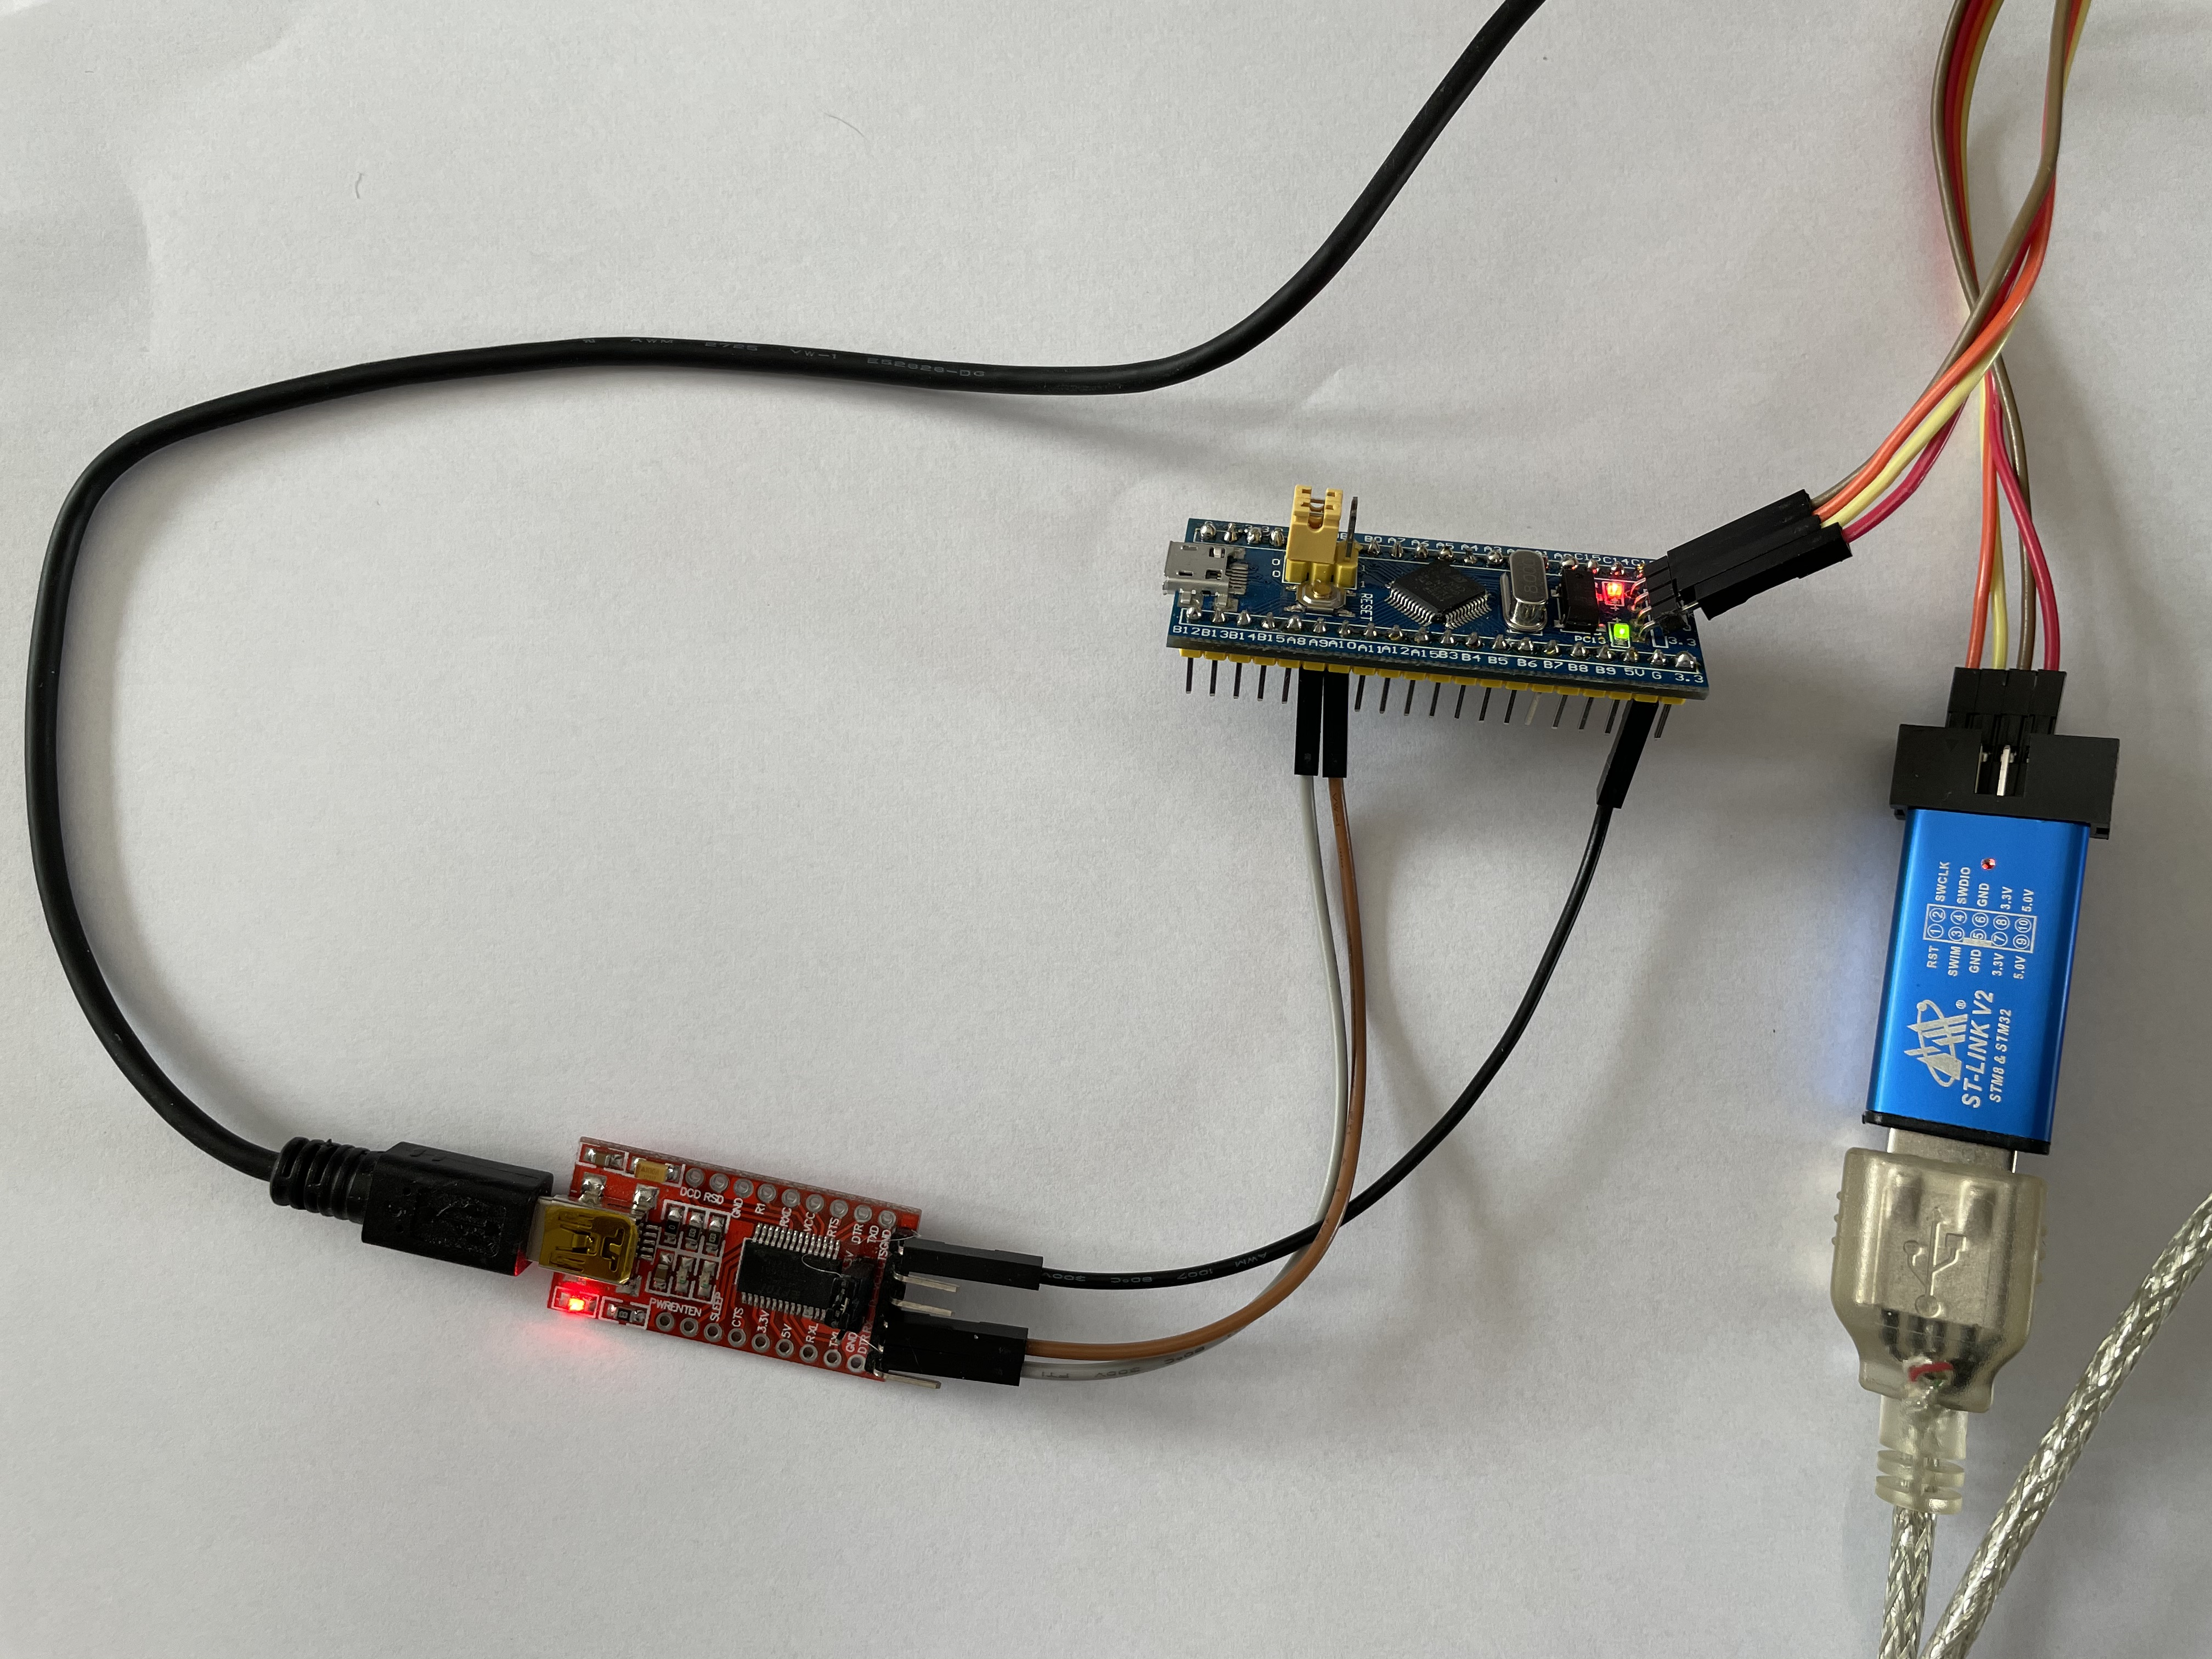
\includegraphics[scale=0.55]{Figures/HardwareSetup_BluePill+STLinkV2+USBSerialAdapter.jpeg}}} % Image background
	\par\normalfont\fontsize{30}{30}\sffamily\selectfont
	\vspace*{1.0cm}
	{\color{blue}
		\textbf{\Huge My "Blue Pill" Projects Test Setup} \\ 
		\textbf{\huge Description and Evaluation} \\
		\vspace*{0.5cm}
		\hspace{-0.3cm}
		{\textbf\huge by Dr. Markus Reinhardt }\par % Book title
		\hspace{-1.3cm}
		{\textbf \huge  \today}\par % Author name
		\vspace*{1.5cm}
	}
\endgroup
\vfill

%%%%%%%%%%%%%%%%%%%%%%%%%%%%%%%%%%%%%%%%%%%%%%%%%%%%%%%%%%%%%%%
% table of contents
\newpage
\thispagestyle{empty}
\tableofcontents
\newpage

%%%%%%%%%%%%%%%%%%%%%%%%%%%%%%%%%%%%%%%%%%%%%%%%%%%%%%%%%%%%%%%
% lists of figures and tables
\newpage
\thispagestyle{empty}
\listoffigures
\listoftables

%%%%%%%%%%%%%%%%%%%%%%%%%%%%%%%%%%%%%%%%%%%%%%%%%%%%%%%%%%%%%%%
% the main text
\newpage
\pagestyle{scrheadings}
\section{Project goals}
The projects are created to test the basic HW / SW concepts for projects based on the so-called "Blue Pill STM32 board".

The used IDE is based on VSCode with PlatformIO extension and STM32 board operated with the Arduino environment.

The HW setup allows to program the board with an ST-Link V2 adapter and also serial communications with a (Linux) PC
via a USB/Serial adapter.

In a second HW setup the control of a LCD via the I2C interface is tested.

In a third project two rotary encoders are used as input devices.

In a fourth project the ADC of the STM32 processor is tested with different resolutions.

The "Blue Pill" STM32 board has a STM32F103C8T6 processor with 20KB RAM and 64KB EEPROM running at 72MHz.
See also \href{https://docs.platformio.org/en/latest//boards/ststm32/bluepill_f103c8.html}{"Blue Pill F103C8" in PlatformIO}.

\section{Project1: Hardware Setup}
A simple HW setup is shown in figure \ref{fig:HWSetup}.
\begin{figure}[htbp]
	\centering
	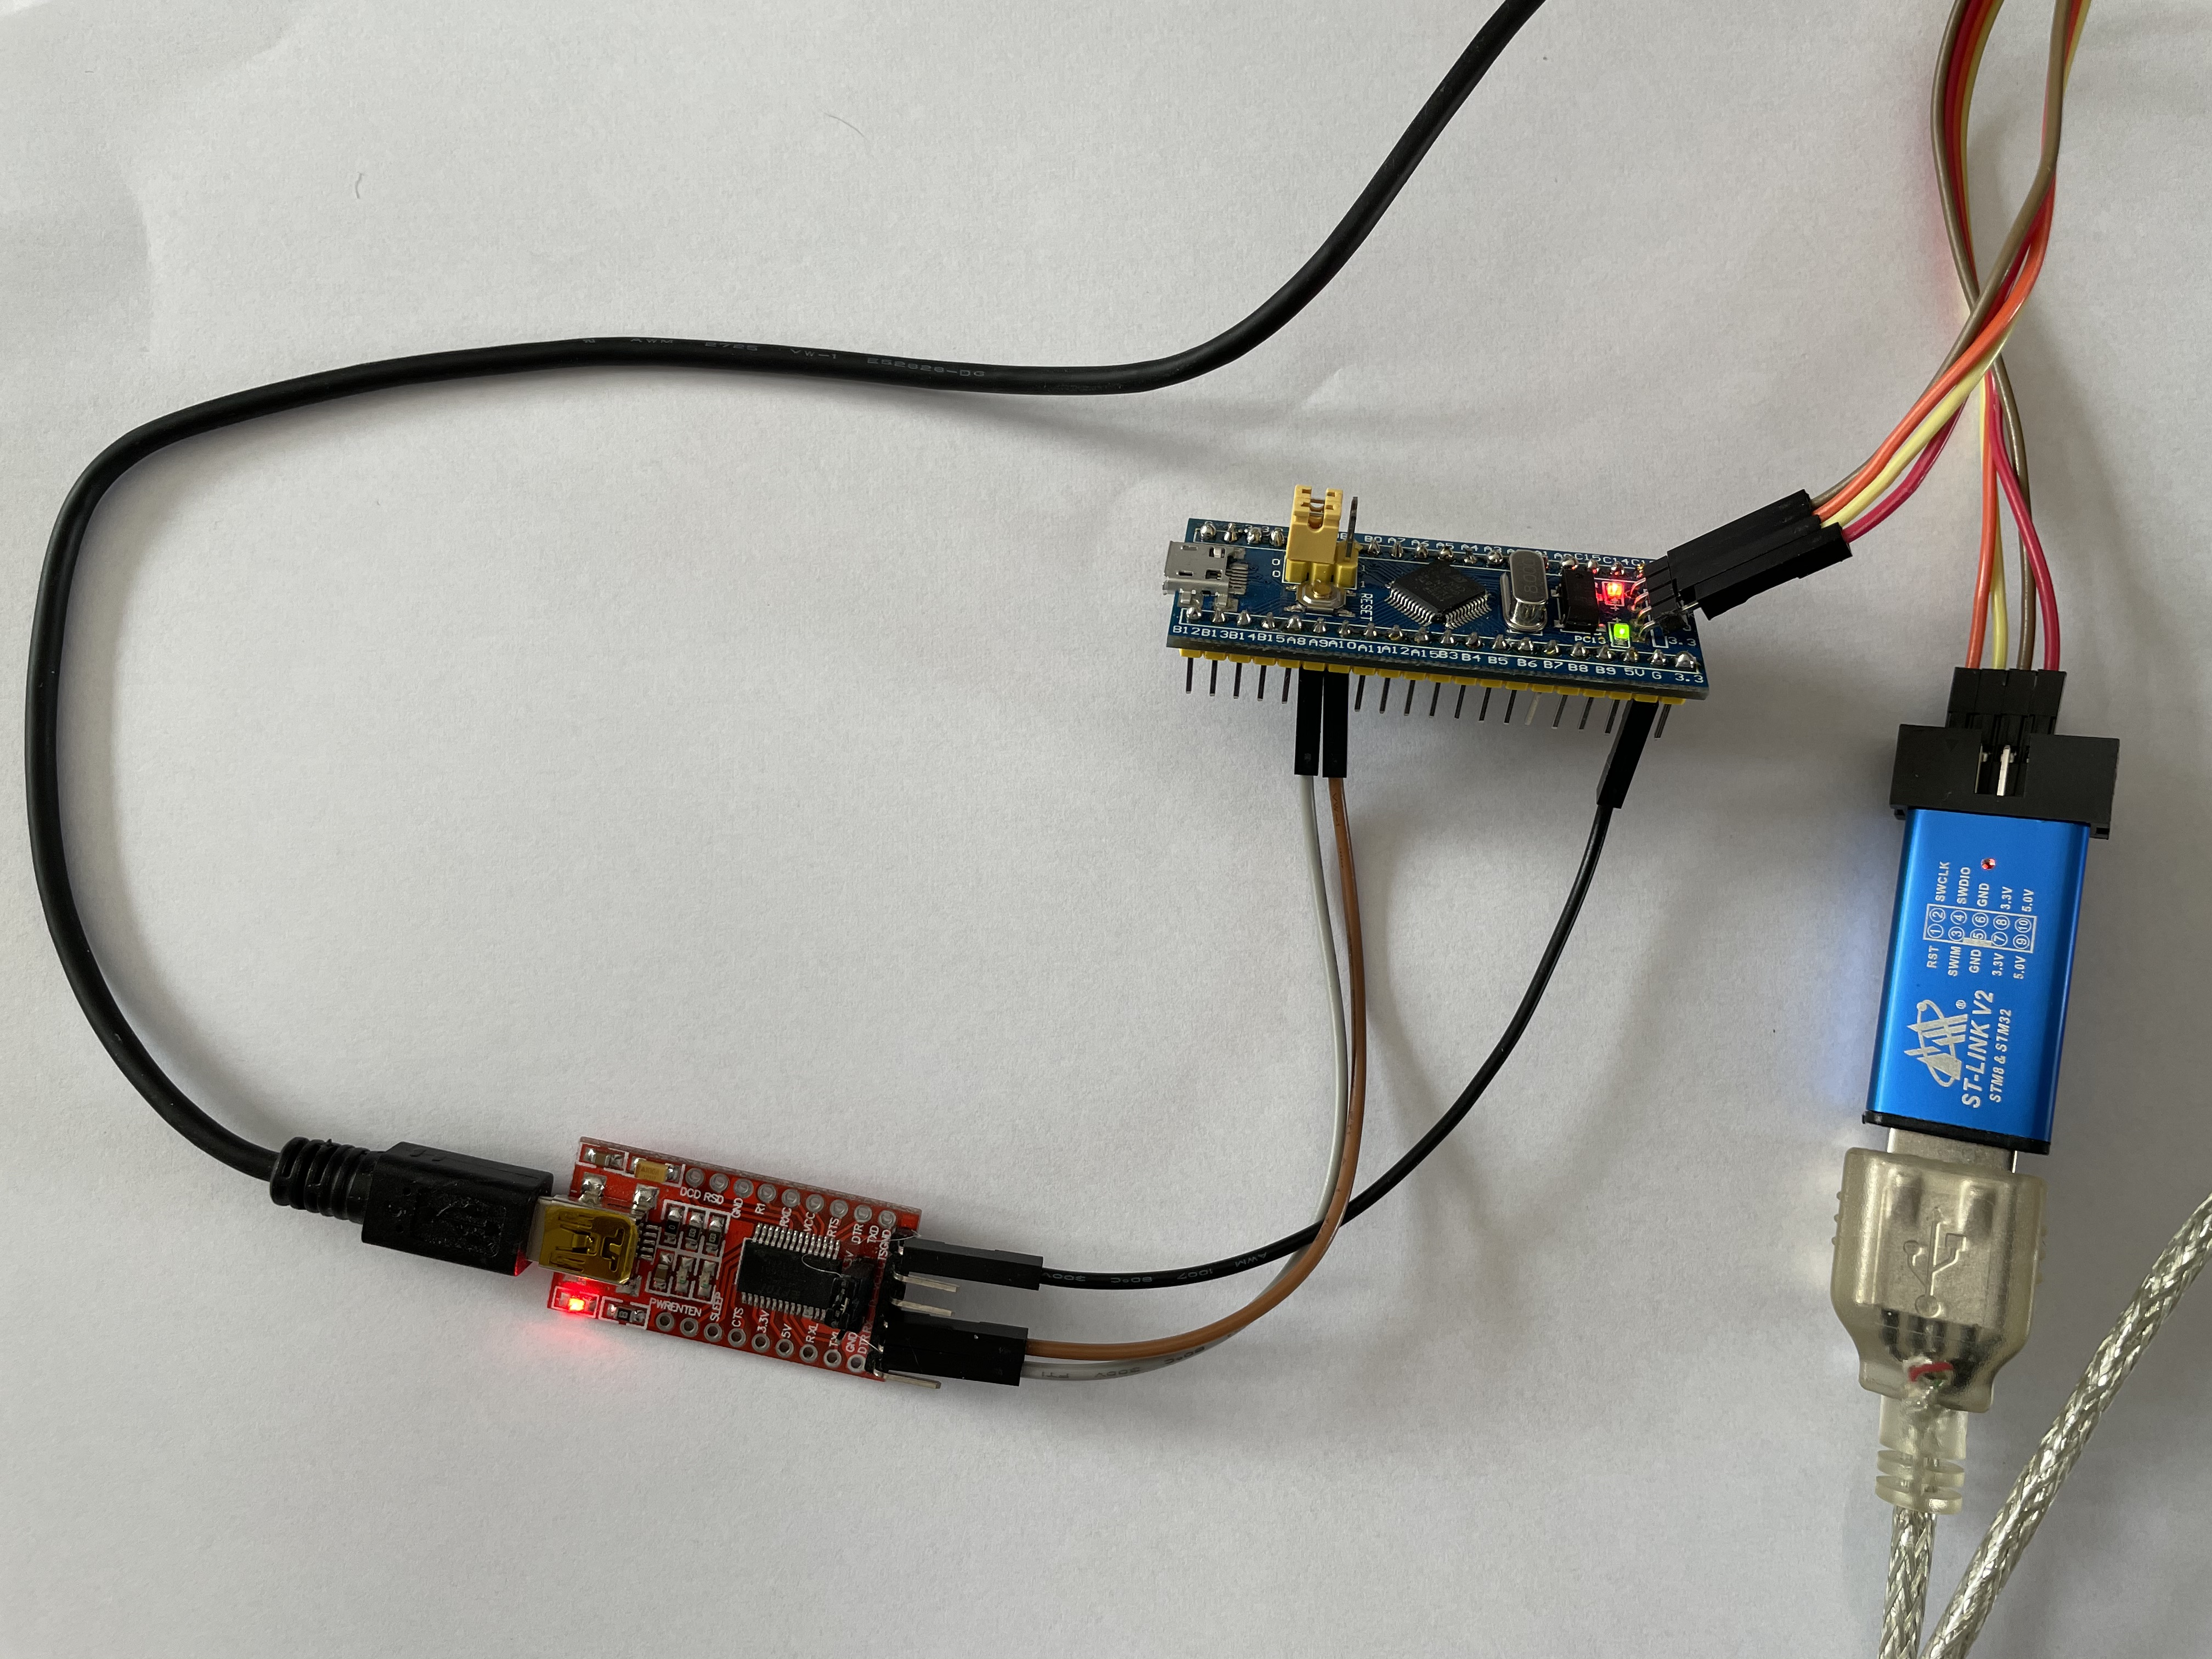
\includegraphics[width=1.0\linewidth]{Figures/HardwareSetup_BluePill+STLinkV2+USBSerialAdapter.jpeg}
	\caption{Project 1 hardware setup}
	\label{fig:HWSetup}
\end{figure}

Note the jumper positions of the two yellow jumpers on the (blue colored) "Blue Pill" board!\\

Programming is done with the (metallic blue colored) ST-Link V2 module. Also the 3.3V power supply for the "Blue Pill" board is delivered by this module.
There are four pins of the module connected with the "Blue Pill" board.
The connections are as follows (Table \ref{table:ConnectionSTLink1}):
\begin{table}[htbp]
\centering
\begin{tabular}{|c|c|c|}
	\hline
	\textbf{Blue Pill} & \textbf{Cable color} & \textbf{ST-Link V2} \\
	\hline
	GND & Brown & GND (Pin 6) \\
	\hline
	3.3V & Red & 3.3V (Pin 8) \\
	\hline
	CLK & Orange & SWCLK (Pin 2) \\
	\hline
	DIO & Yellow & SWDIO (Pin 4) \\
	\hline
\end{tabular}
\caption{Connection "Blue Pill" to ST-Link V2}
\label{table:ConnectionSTLink1}
\end{table}

A USART interfacing between the Blue Pill board and the PC / IDE is realized with the (red colored) USB/Serial adapter board.
Note the jumper position on the board is such that the 3.3V output voltage is provided (but not connected in this setup) as the "Blue
Pill" processor is operated with 3.3V. In the software the Arduino Serial1 interface port is used.
The connection between the USB/Serial adapter and the Blue Pill board is done as follows (Table \ref{table:ConnectionSerial1}):
\begin{table}[htbp]
\centering
\begin{tabular}{|c|c|c|}
	\hline
	\textbf{Blue Pill} & \textbf{Cable color} & \textbf{USB/Serial} \\
	\hline
	GND & Black & GND \\
	\hline
	TX1 (Pin PA9) & Gray & RX \\
	\hline
	RX1 (Pin PA10) & Brown & TX \\
	\hline
\end{tabular}
\caption{Connection "Blue Pill" to USB/Serial adapter}
\label{table:ConnectionSerial1}
\end{table}

The USB/Serial adapter appears under /dev/ttyUSB0 in the Linux operating system. This port has to be selected in the IDE, when the Serial Monitor is activated.

\section{Project 1: PlatformIO IDE }
The IDE for project 1 with the first Arduino sketch is shown in figure \ref{fig:IDESetup}.
\begin{figure}[htbp]
	\centering
	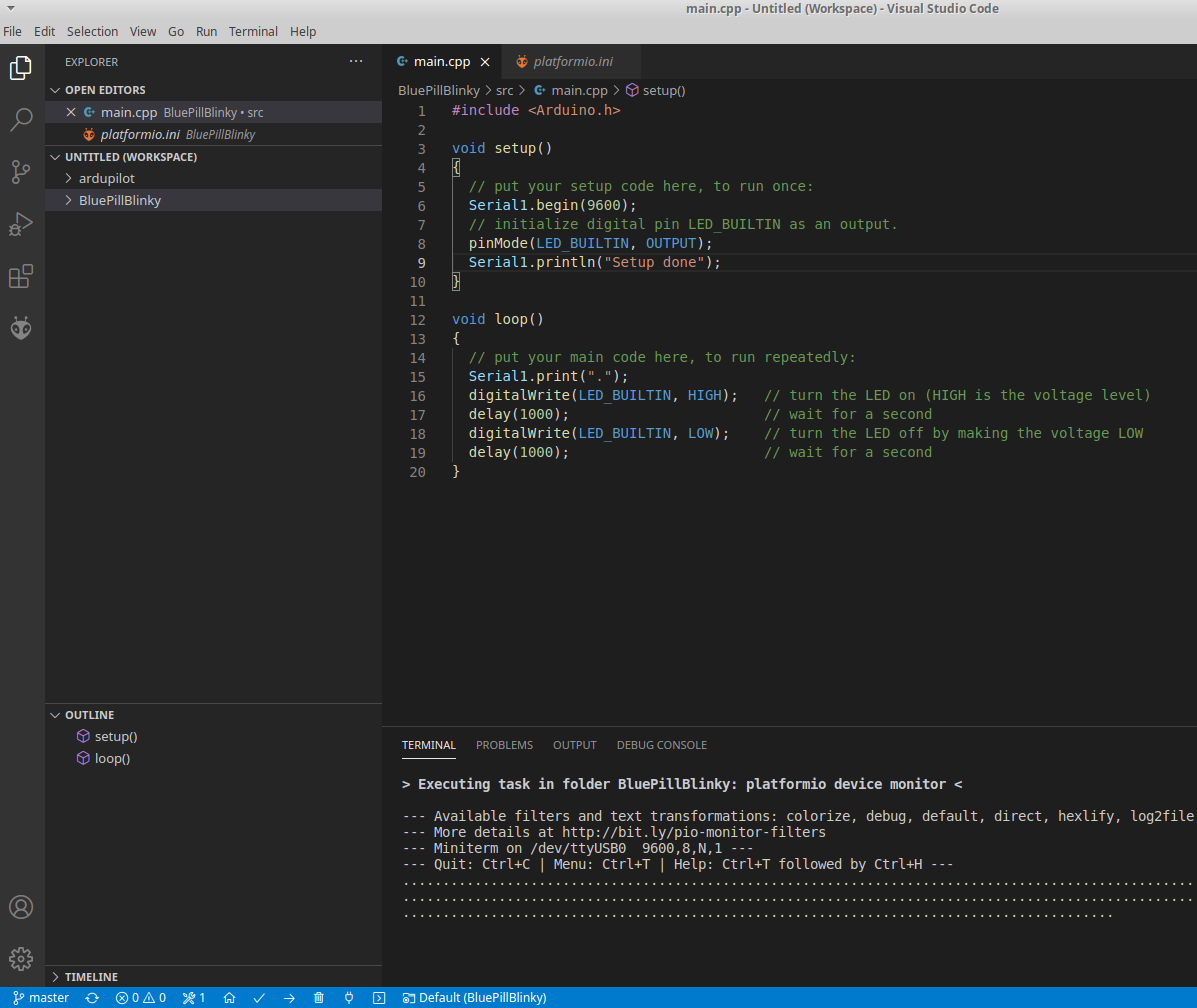
\includegraphics[width=1.0\linewidth]{Figures/VSCode+PlatformIO+SerialMonitor+Blinky.png}
	\caption{VSCode/PlatformIO (Arduino environment) IDE}
	\label{fig:IDESetup}
\end{figure}
The picture shows the PlatformIO IDE within the VSCode editor and the main Arduino sketch which implements the simple blinking of the on-board LED and the output of data via the Serial1 port.

The picture also shows the output of dots (see the sketch code) via the USB/Serial adapter and the Serial1 Arduino interface
to the Arduino Serial Monitor displayed in the lower part of the IDE.\\

The development cycle is controlled by pressing the relevant buttons in the blue bottom line of the IDE (see the call-outs of the buttons when moving over them with the mouse pointer).\\

\textbf{Important Note}: If you have multiple projects within the Platform IDE, do not forget to select the right project in the bottom line (in the figure here:
"Default (BluePillBlinky)") before compiling.\\

Compilation is done by pressing the "Check" button.

Program download is done by pressing the "Right Arrow" button.

Activation of the Serial Arduino Monitor is done with the "Plug" button.

To switch back to the PlatfromIO home screen is done with the "Home" button. 

\newpage
\section{Project 2: LCD control via I2C}
The IDE with the second Arduino sketch is shown in figure \ref{fig:IDESetup2}.
\begin{figure}[htbp]
	\centering
	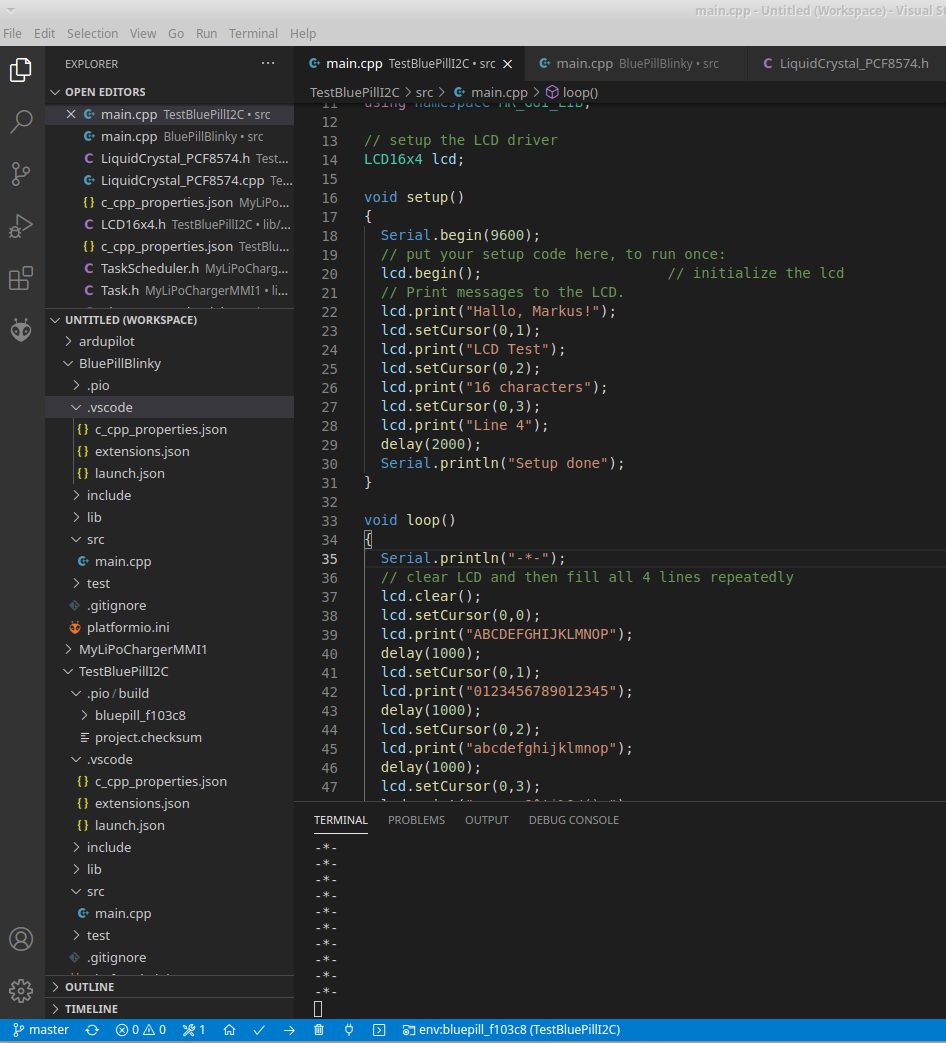
\includegraphics[width=0.85\linewidth]{Figures/Test_BluePill_I2C_LCD_IDE.png}
	\caption{VSCode/PlatformIO IDE}
	\label{fig:IDESetup2}
\end{figure}
The sketch controls a 16x4 character LCD connected to the "Blue Pill" board via the I2C interface.\\
In this sketch the Serial Arduino interface is used for test messages to the Serial Monitor of the IDE. It is connected to pins PA9 (TX1) and PA10 (RX1) and via the USB/Serial adapter to the PC. The IDE shows in the lower part the Serial Monitor and the messages received from the "Blue Pill" board.\\

The HW setup for this test is shown in figure \ref{fig:HWSetupI2CLCD}
\begin{figure}[htbp]
	\centering
	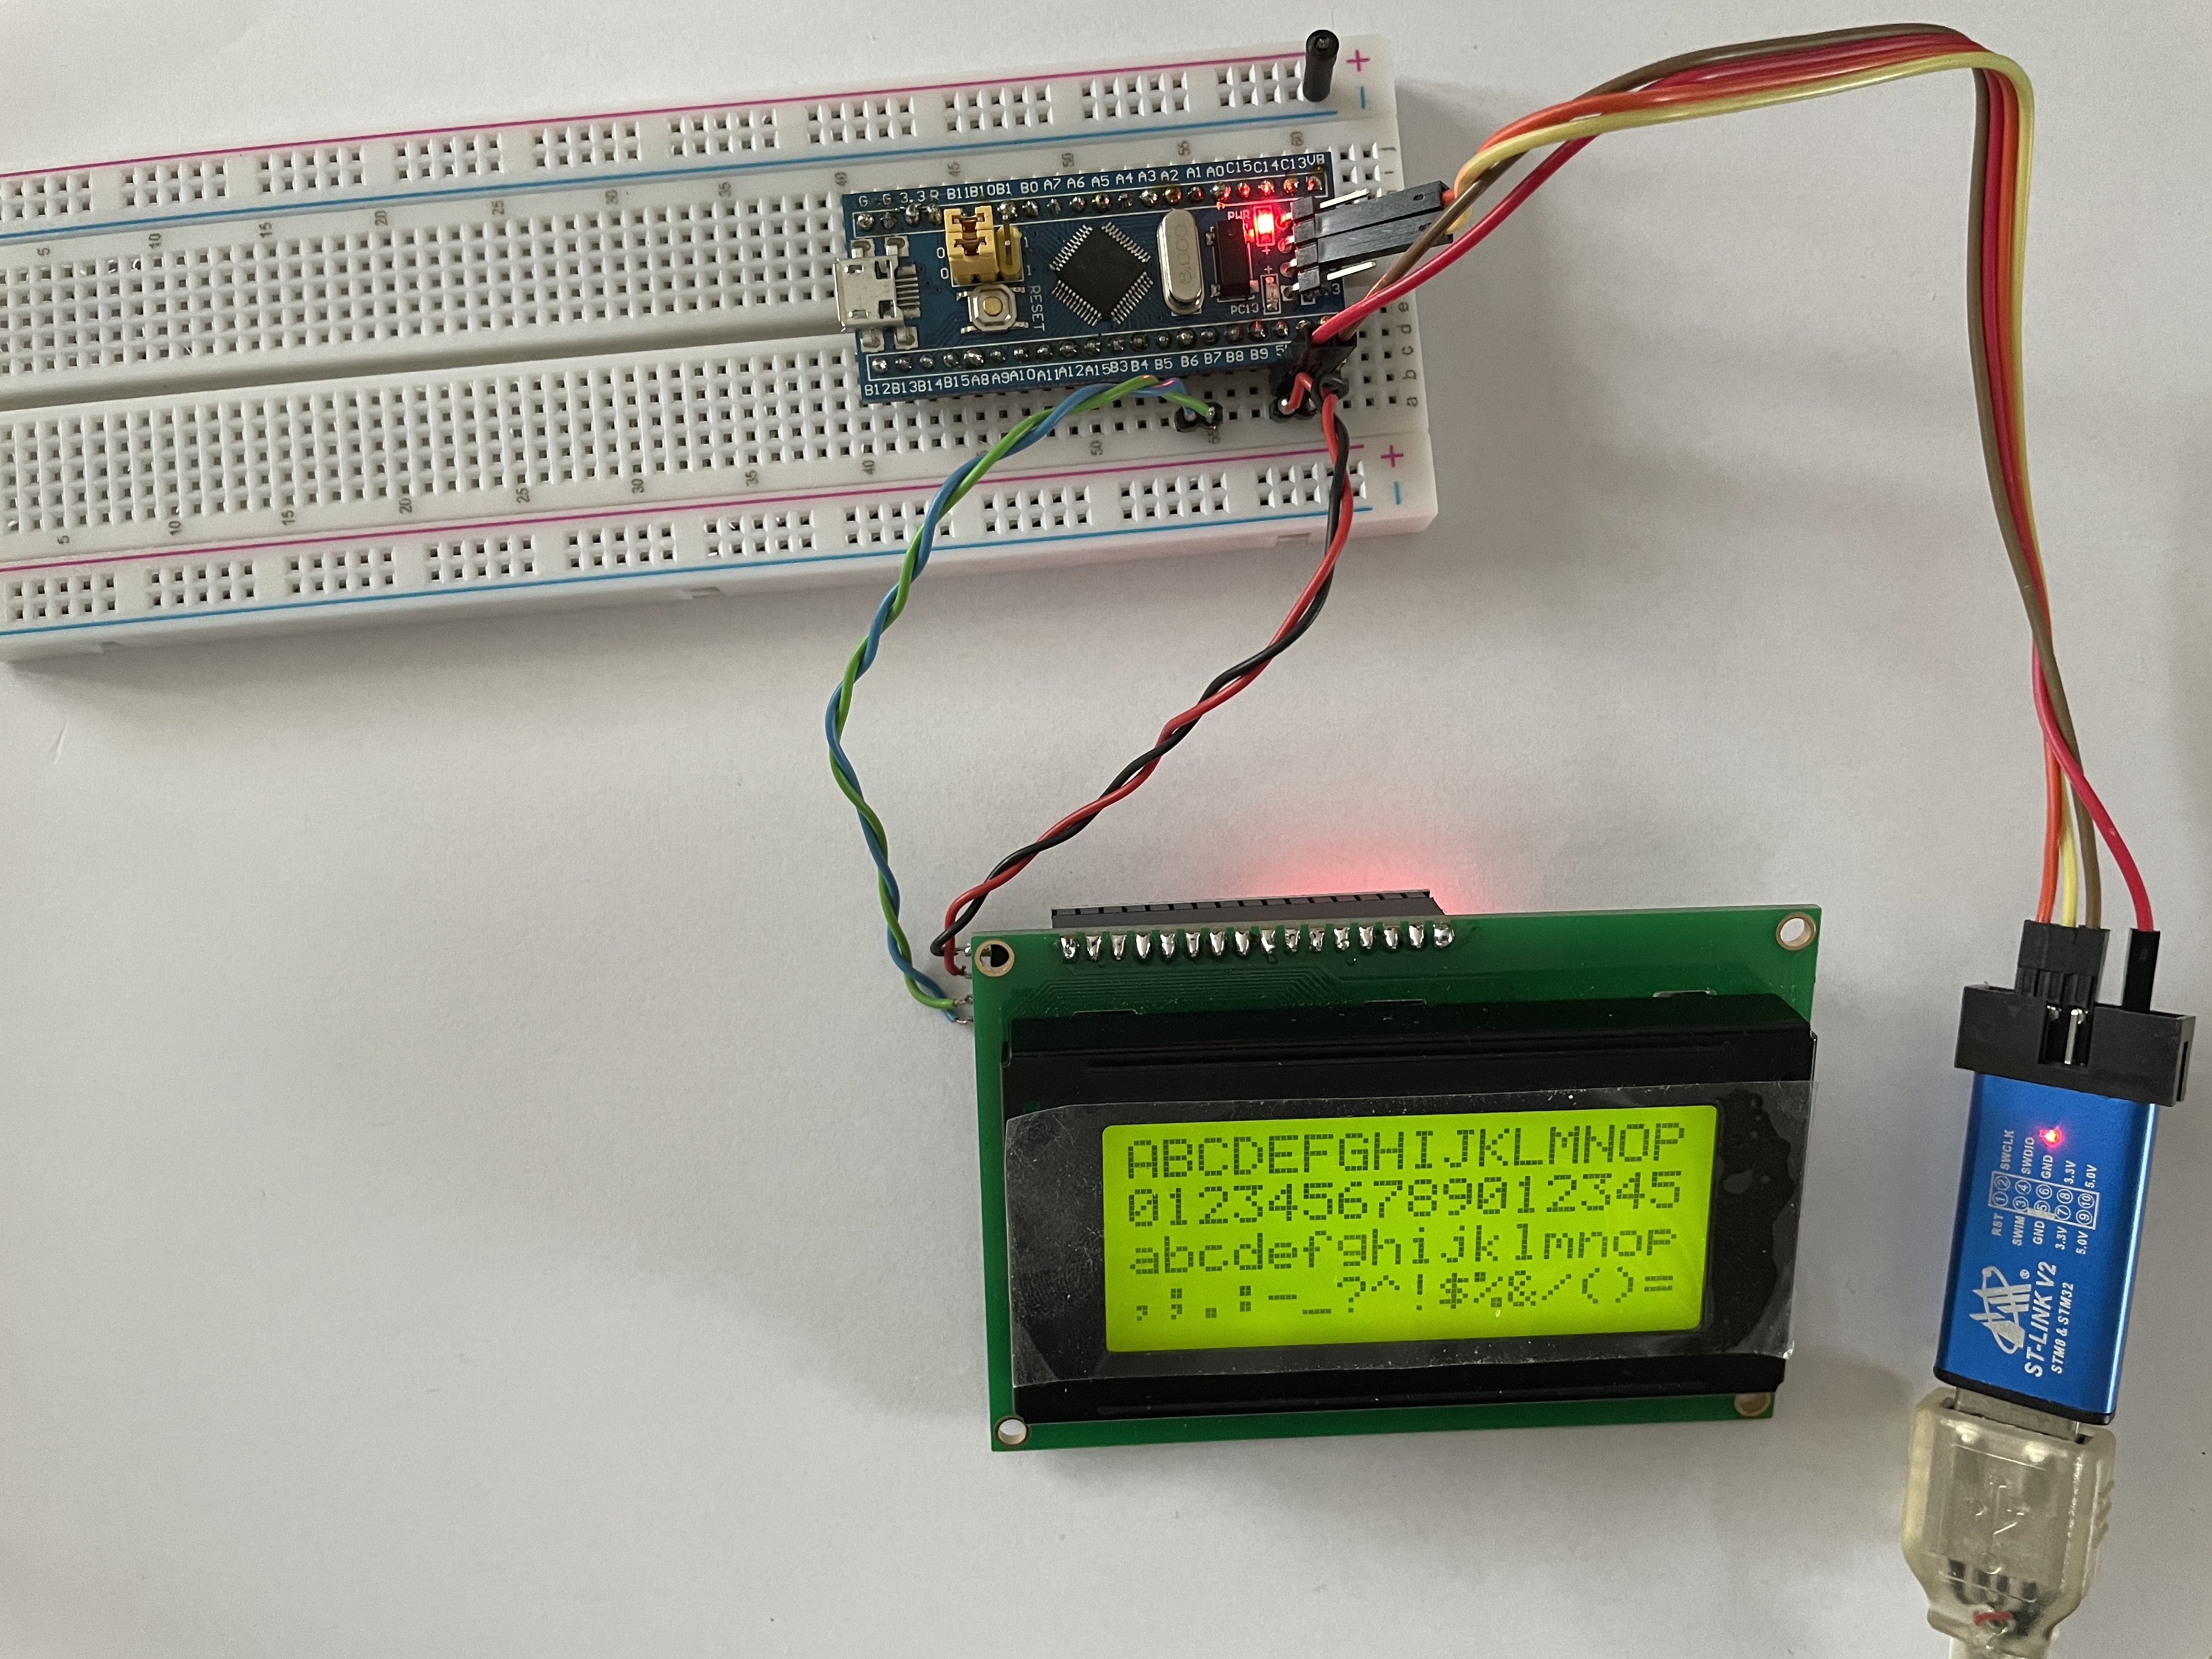
\includegraphics[width=1.0\linewidth]{Figures/Test_BluePill_I2C_LCD_HWSetup.jpeg}
	\caption{Project 2 HW setup with I2C-LCD}
	\label{fig:HWSetupI2CLCD}
\end{figure}
The connection from the ST-Link V2 adapter to the "Blue Pill" board is now using the 5V pins according to the following table
(Table \ref{table:ConnectionSTLink2}).
The 3.3V for the processor is now provided by the on-board fixed power regulator. The 5V power supply is also required for the LCD.
\begin{table}[htbp]
	\centering
	\begin{tabular}{|c|c|c|}
		\hline
		\textbf{Blue Pill} & \textbf{Cable color} & \textbf{ST-Link V2} \\
		\hline
		GND & Brown & GND (Pin 6) \\
		\hline
		5V & Red & 5V (Pin 10) \\
		\hline
		CLK & Orange & SWCLK (Pin 2) \\
		\hline
		DIO & Yellow & SWDIO (Pin 4) \\
		\hline
	\end{tabular}
\caption{Connection "Blue Pill" to USB/Serial adapter}
\label{table:ConnectionSTLink2}
\end{table}
The connection between the "Blue Pill" board and the I2C adapter of the LCD is done here as follows (Table \ref{table:ConnectionI2C}):
\begin{table}[htbp]
	\centering
	\begin{tabular}{|c|c|c|}
		\hline
		\textbf{Blue Pill} & \textbf{Cable color} & \textbf{I2C LCD} \\
		\hline
		GND & Black & GND \\
		\hline
		5V & Red & 5V \\
		\hline
		SCL1 (Pin PB6) & Blue & SCL \\
		\hline
		SDA1 (Pin PB7) & Green & SDA \\
		\hline
	\end{tabular}
\caption{Connection "Blue Pill" to I2C adapter of the LCD}
\label{table:ConnectionI2C}
\end{table}
The connection between the "Blue Pill" board and the USB/Serial adapter is equal to setup 1 (Table \ref{table:ConnectionSerial1}).

\newpage
\section{Project 3: Test of Rotary Encoders}
Figure \ref{fig:BluePillRotEnc} shows the test of two rotary encoders  at the "Blue Pill" board.
\begin{figure}[htbp]
	\centering
	\includegraphics[width=0.8\linewidth]{Figures/Test_BluePill_RotaryEncoder.jpeg}
	\caption{Rotary encoder test at the "Blue Pill" board}
	\label{fig:BluePillRotEnc}
\end{figure}
The connection of the rotary encoders is done according to the following tables
\ref{table:ConnectionRotEnc1}, \ref{table:ConnectionRotEnc2} ):
\begin{table}[htbp]
	\centering
	\begin{tabular}{|c|c|c|}
		\hline
		\textbf{Blue Pill} & \textbf{Cable color} & \textbf{rotary encoder 1} \\
		\hline
		GND & Black & GND \\
		\hline
		5V & Red & 5V \\
		\hline
		Pin PB12 & White & SW \\
		\hline
		Pin PB13 & Blue & DT \\
        \hline
  		Pin PB14 & Yellow & CLK \\
		\hline
	\end{tabular}
\caption{Connection "Blue Pill" to rotary encoder 1}
\label{table:ConnectionRotEnc1}
\end{table}

\begin{table}[htbp]
	\centering
	\begin{tabular}{|c|c|c|}		
	\hline
		\textbf{Blue Pill} & \textbf{Cable color} & \textbf{rotary encoder 2} \\
		\hline
		GND & Black & GND \\
		\hline
		5V & Red & 5V \\
		\hline
		Pin PB3 & White & SW \\
		\hline
		Pin PB4 & Blue & DT \\
		\hline
		Pin PB5 & Green & CLK \\
		\hline
	\end{tabular}
	\caption{Connection "Blue Pill" to rotary encoder 2}
	\label{table:ConnectionRotEnc2}
\end{table}
A key press or a turn of a rotary encoder creates a HW interrupt on the processor. The specific interrupt service routines evaluate the key hits and determine the turn direction.

\newpage
\section{Project 4: Test of the ADC}
The ADC of the "Blue Pill processor in the Arduino environment can be programmed to use for the resolution a different number of bits. 
Figure \ref{fig:BluePillADC} shows the ADC characteristic of the "Blue Pill" processor for the 10bit and 12bit cases.
\begin{figure}[htbp]
	\centering
	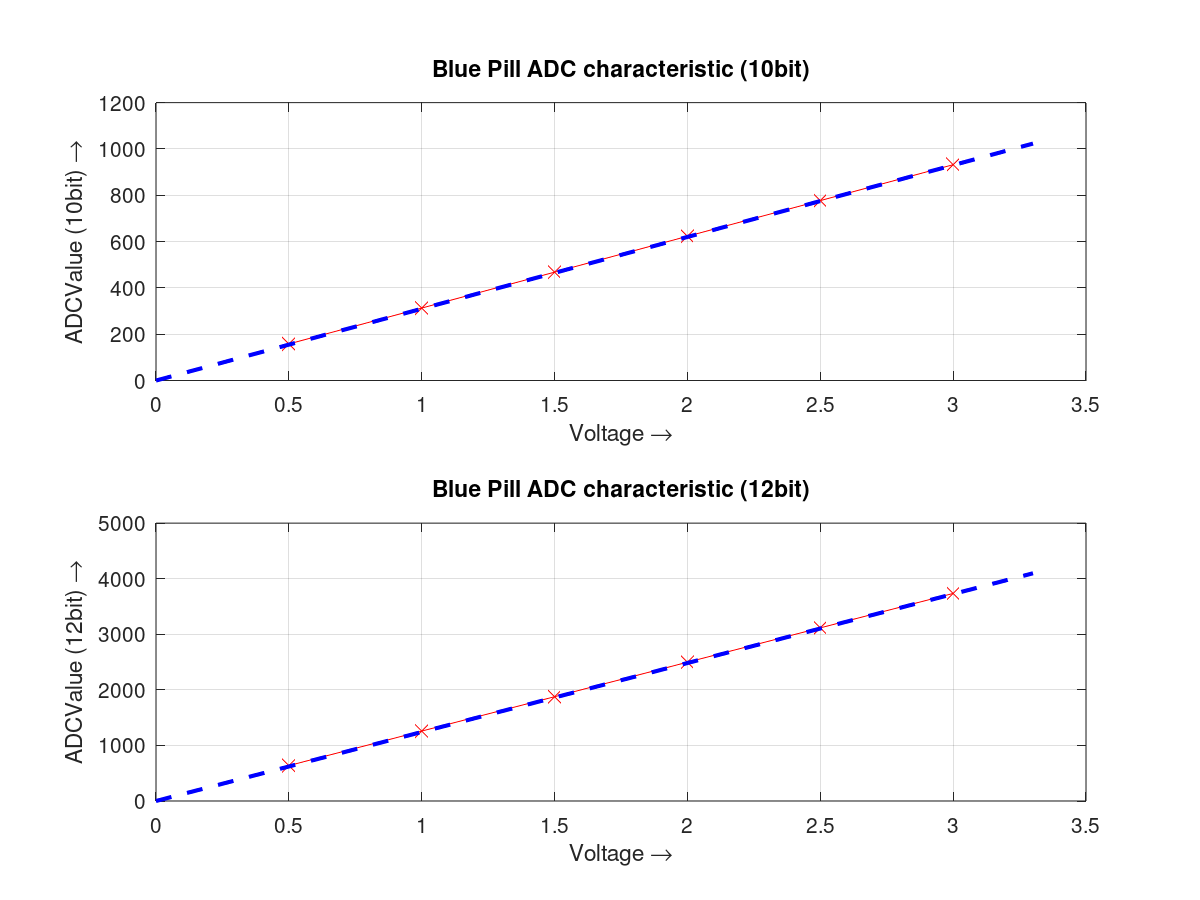
\includegraphics[width=0.9\linewidth]{Figures/BluePillADCCharacteristic.png}
	\caption{ADC characteristic of the "Blue Pill" processor}
	\label{fig:BluePillADC}
\end{figure}
The figures show in red color the measured ADC characteristic and in blue the ideal linear ADC characteristics.
The ADC reference voltage ($V_{ref}$) is equal to the power supply voltage of the processor of 3.3V.
The ADC value is given the as follows:\\
For the 10bit ADC resolution case:
\begin{equation*}
 \text{ADCValue} = \text{voltage (at ADC pin Ax)} ~/~ V_{ref} \cdot 1024
\end{equation*}
For the 12bit ADC resolution case:
\begin{equation*}
\text{ADCValue} = \text{voltage (at ADC pin Ax)} ~/~ V_{ref} \cdot 4096
\end{equation*}

\newpage
\section{Project 5: Test of PWM}
The STM32 processor of the "Blue Pill" board has multiple PWM capable pins.
Figure \ref{fig:BluePillPWM} shows the generated PWM signal of the "Blue Pill" processor on the screen of a hand-held oscilloscope.
\begin{figure}[htbp]
	\centering
	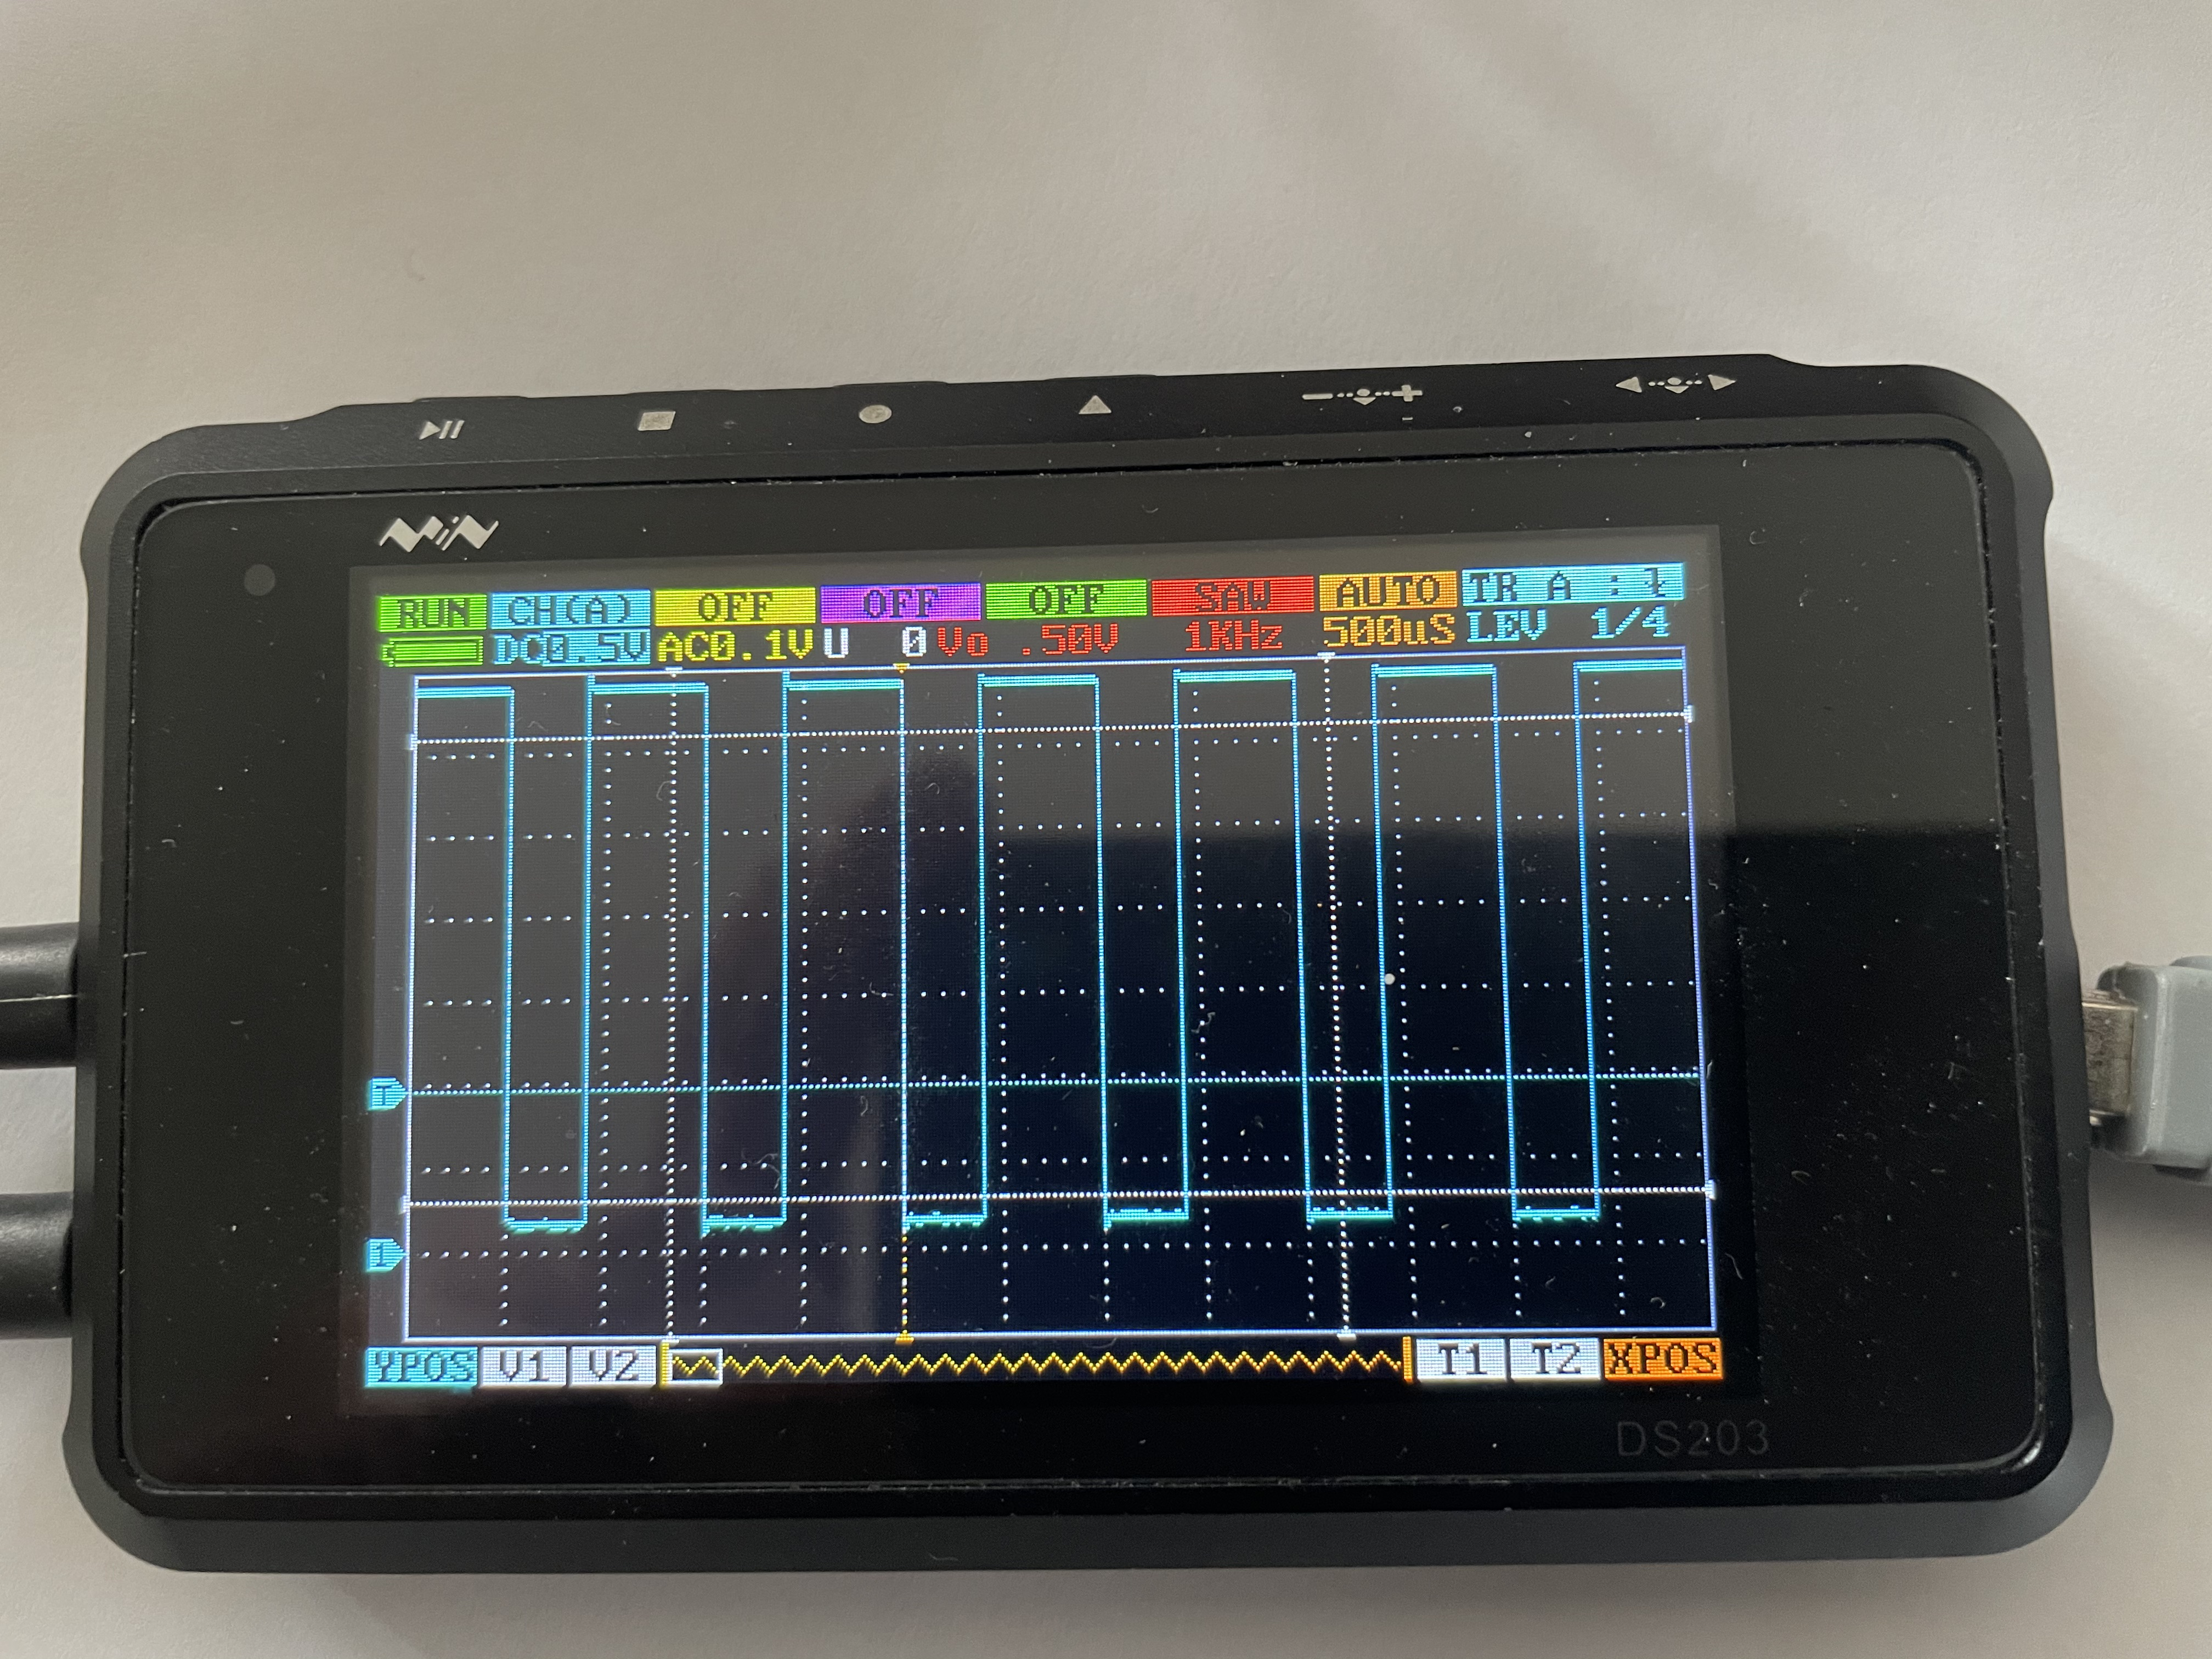
\includegraphics[width=0.9\linewidth]{Figures/Test_BluePill_PWM.jpeg}
	\caption{PWM signal of the "Blue Pill" processor}
	\label{fig:BluePillPWM}
\end{figure} 

\newpage
\appendix
\section{Appendix A}
\subsection{Pin-out of the "Blue Pill" board}
Figure \ref{fig:BluePillPinout} shows the pin-out of the "Blue Pill" board.
\begin{figure}[htbp]
	\centering
	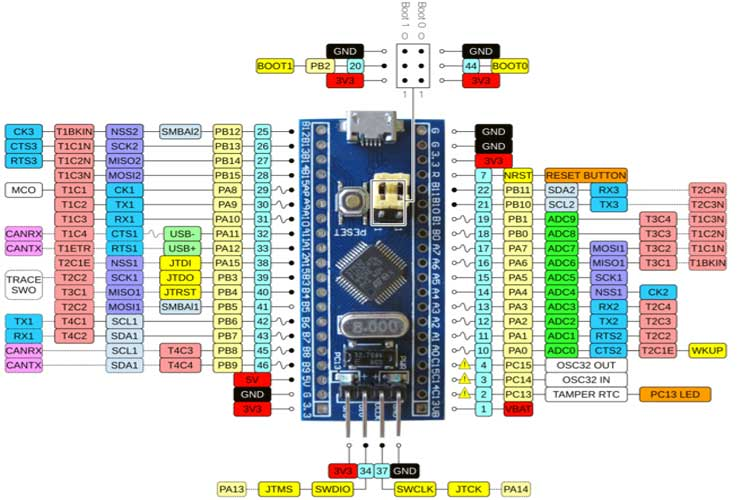
\includegraphics[width=1.0\linewidth]{Figures/STM32-Blue-Pill-Development-Board-Pinout.jpg}
	\caption{Pin-out of the "Blue Pill" board}
	\label{fig:BluePillPinout}
\end{figure}

\subsection{Helpful Links}
\href{https://platformio.org/platformio-ide}{PlatformIO IDE}\\
\href{https://docs.platformio.org/en/latest//boards/ststm32/bluepill_f103c8.html}{"Blue Pill F103C8" in PlatformIO}\\
\href{https://www.youtube.com/watch?v=cmHQxd_qGl8}{Installing PlatformIO and creating a sample program for STM32 Blue Pill}\\
\href{https://www.arduino.cc/en/Tutorial/HomePage}{Arduino Getting Started and Tutorials}

\end{document}